\section{Adding Flow in Flow Table}

\subsection{Overview}
\begin{wrapfigure}{l}{0.45\textwidth} \vspace{-20pt}
\begin{center}
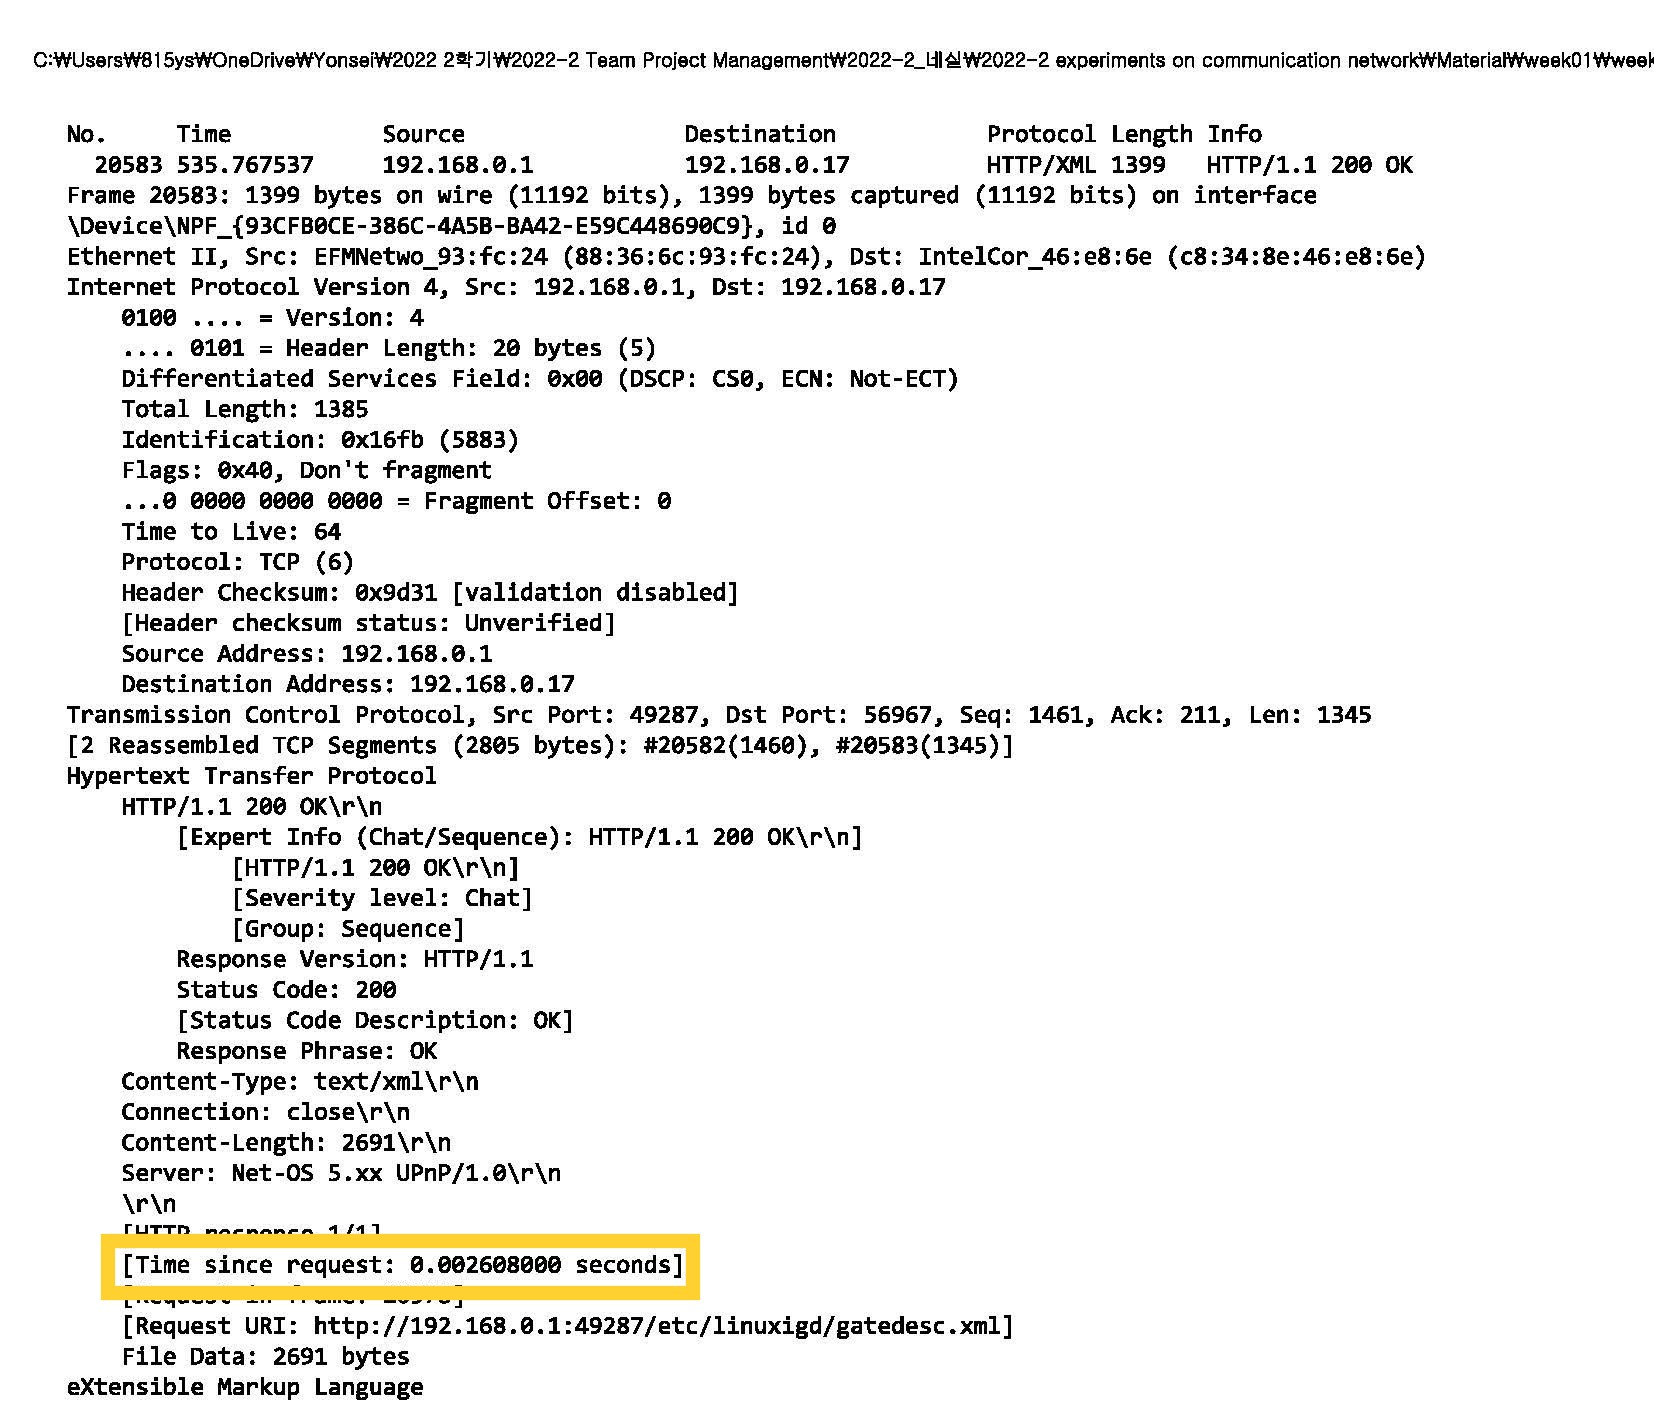
\includegraphics[width=0.3\textwidth]{image/result_week01/Q1-2.jpg}    
\end{center}
\end{wrapfigure}
blabla

\subsection{Experiment Results}
\subsubsection{Flow Table}
\begin{figure}[!h]\centering 
	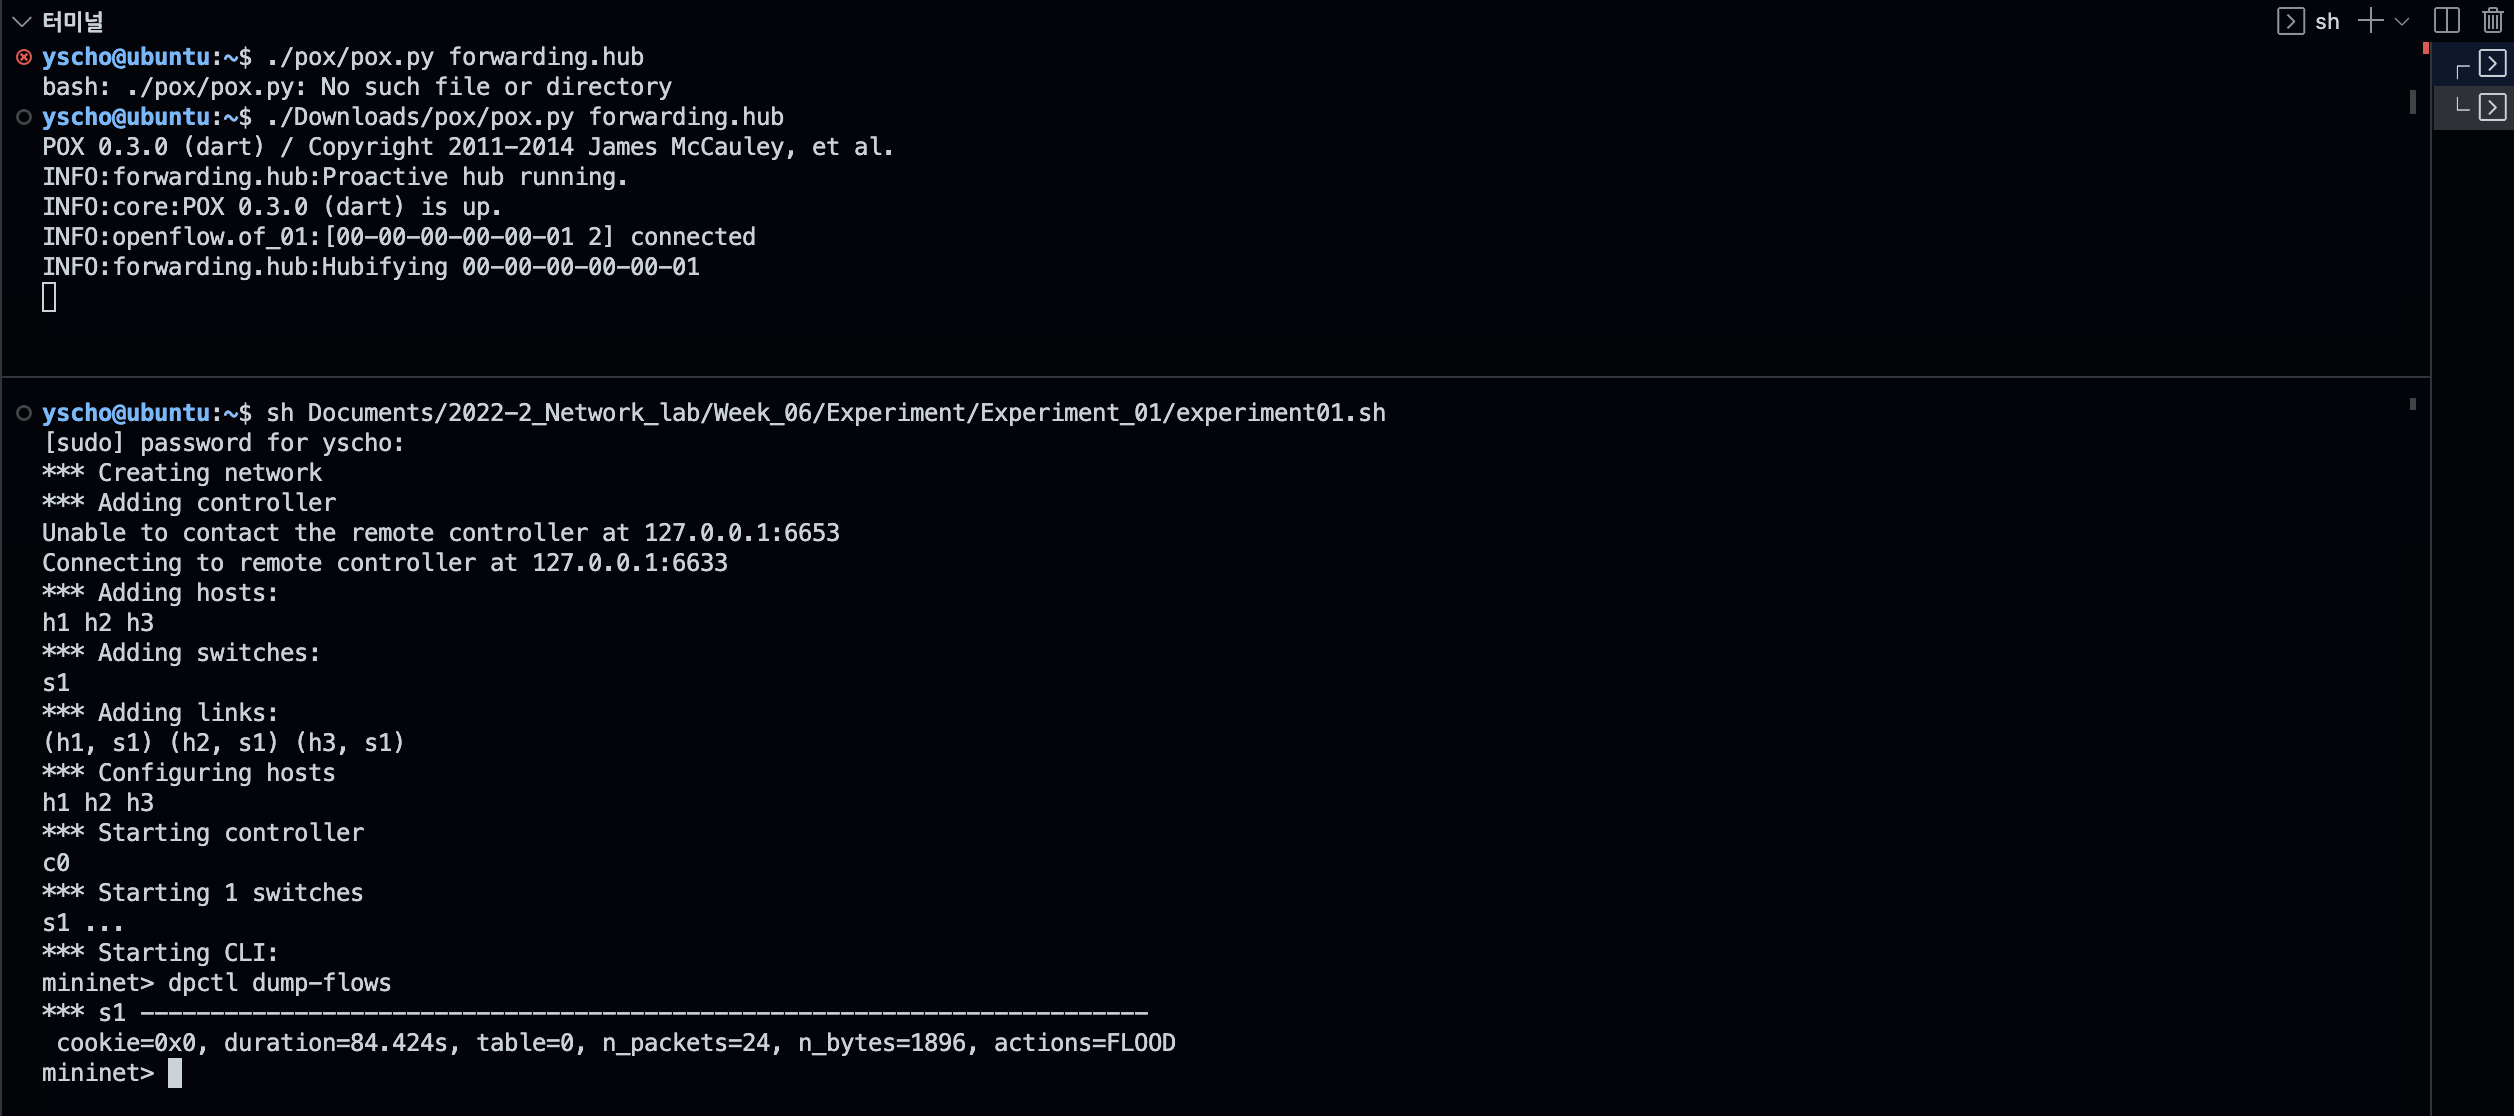
\includegraphics[width=.99\textwidth]{image/week06/2-1.png}
	\caption{\footnotesize 
	Simulation Scenario of topology used in week 06 experiment}
	\vspace{-10pt}
\end{figure}
\subsubsection{Ping Test}
\begin{figure}[h!]
\centering
\subfloat[]{
    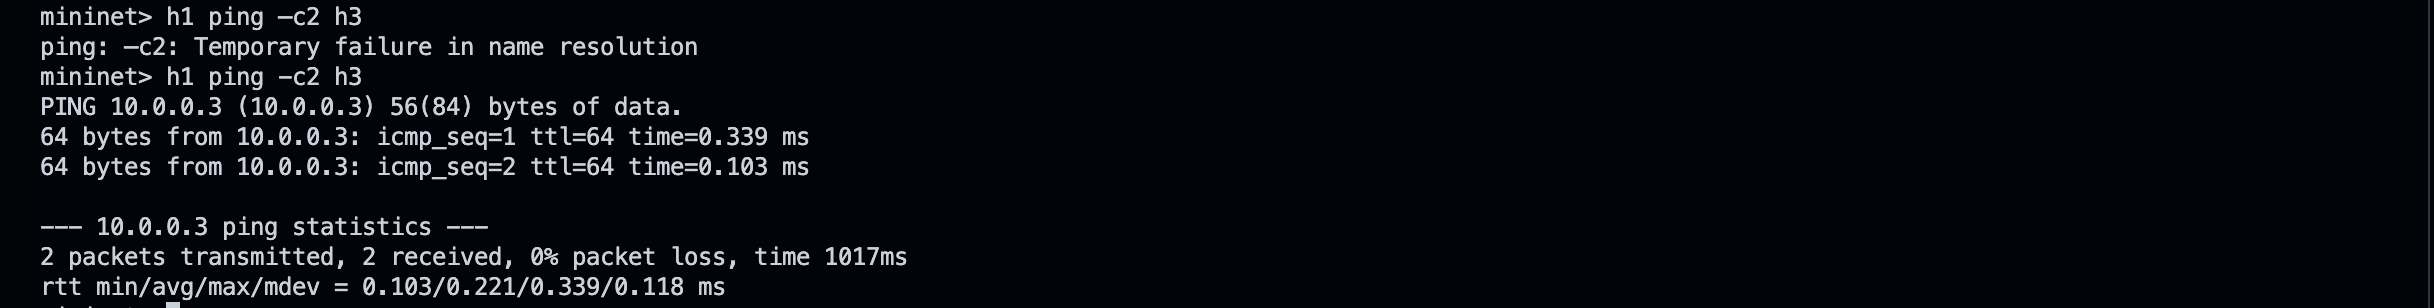
\includegraphics[width=0.99\textwidth]{image/week06/2-2-1.png}
}
\hfill
\subfloat[]{
    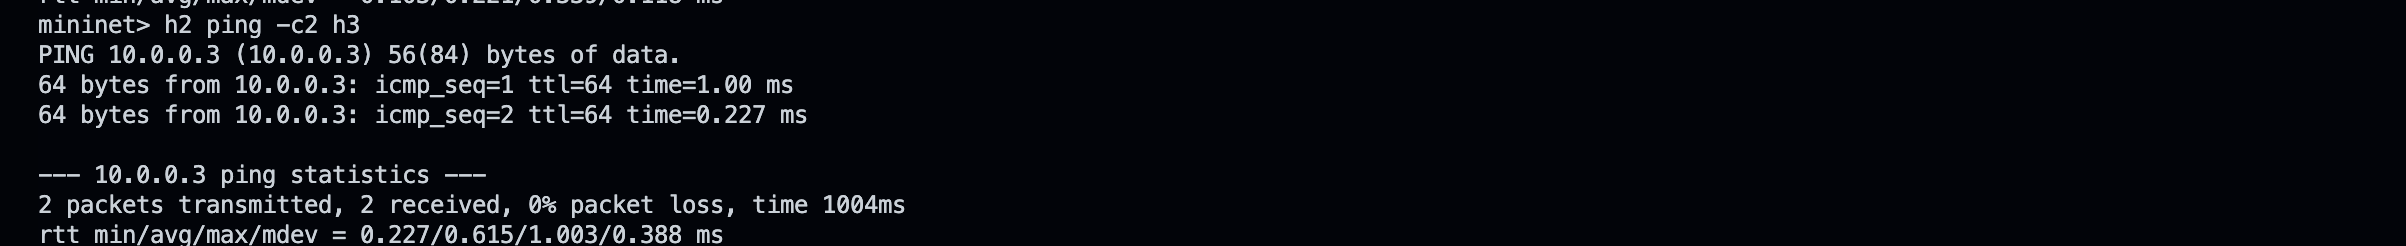
\includegraphics[width=0.99\textwidth]{image/week06/2-2-2.png}
}\caption{}
\end{figure}

\clearpage
\subsubsection{Interface Listeing}
\begin{figure}[h!]
\centering
\subfloat[Screenshot of h1's terminal]{
    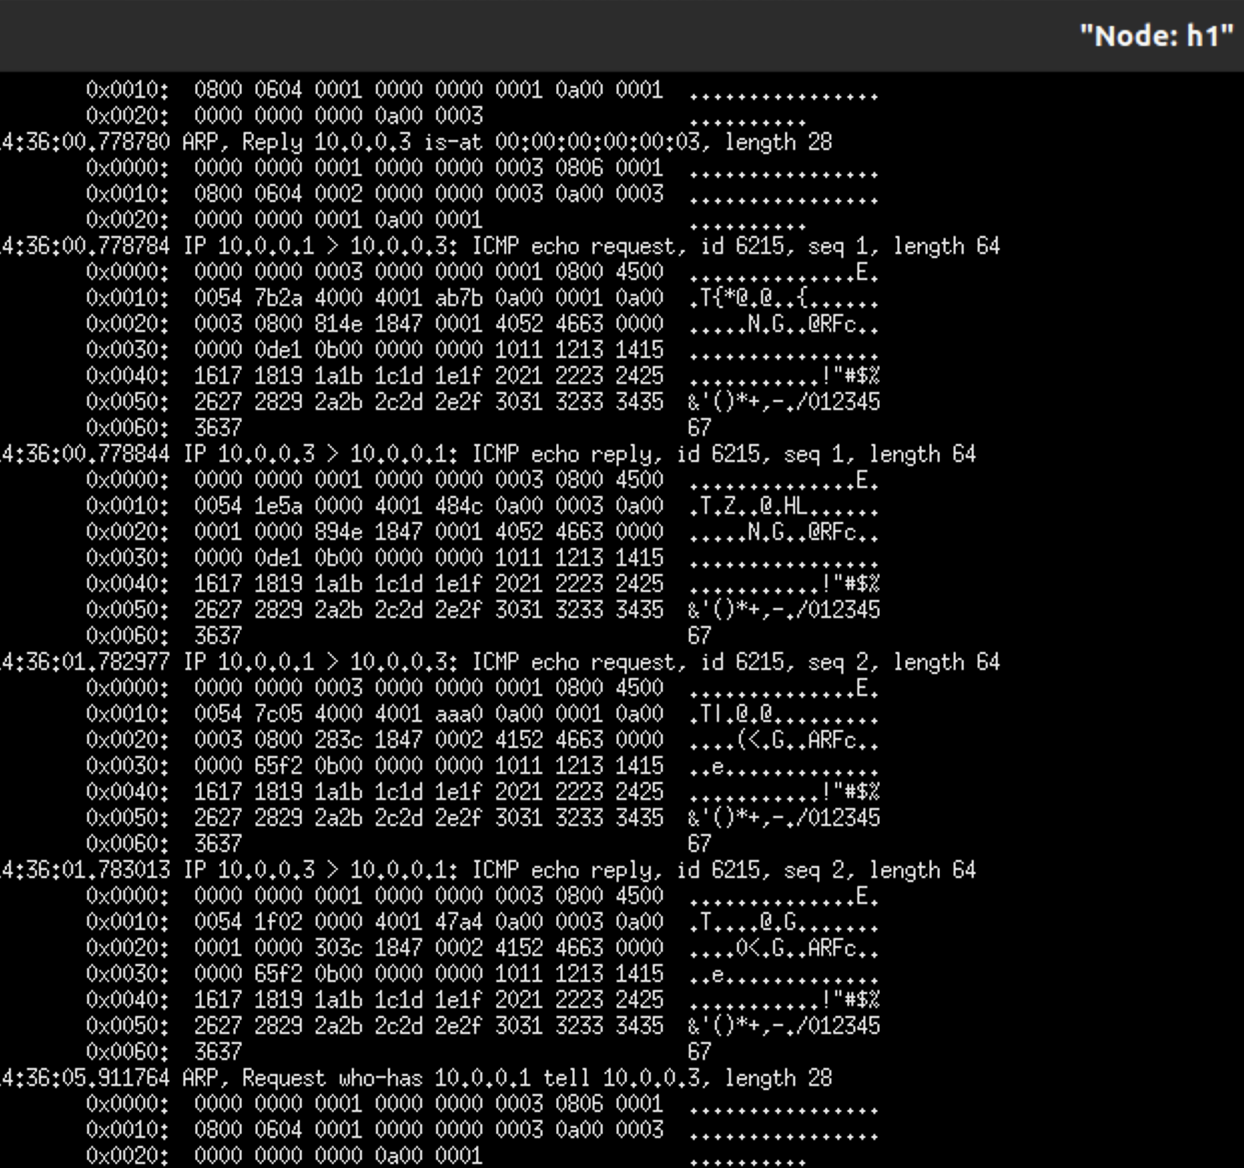
\includegraphics[width=0.33\textwidth]{image/week06/2-3-1.png}
}
\subfloat[Screenshot of h2's terminal]{
    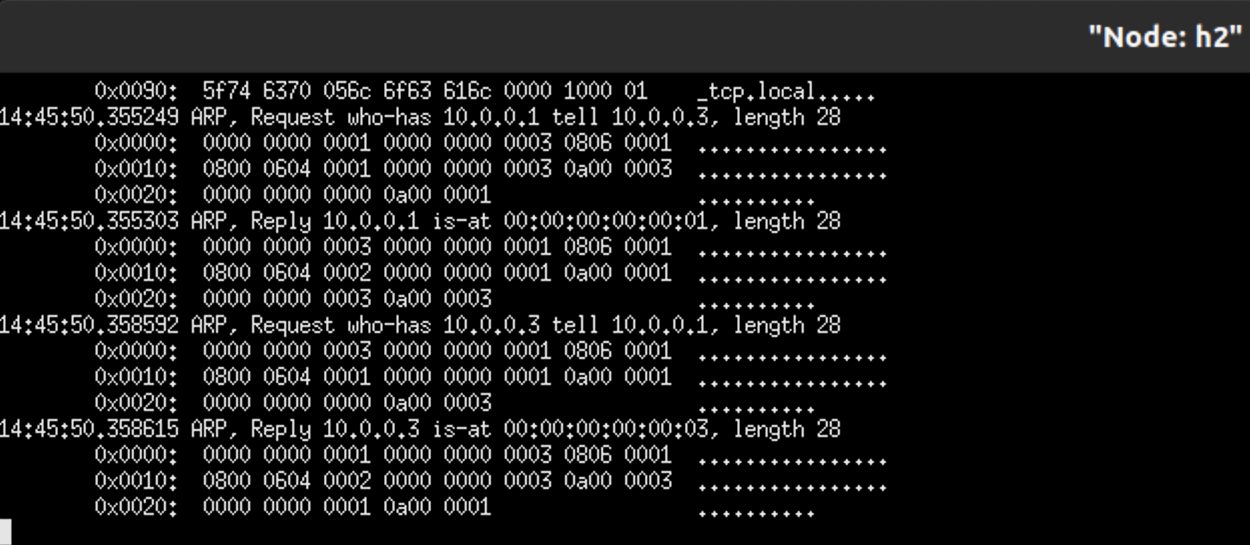
\includegraphics[width=0.33\textwidth]{image/week06/2-3-2.png}
}
\subfloat[Screenshot of h3's terminal]{
    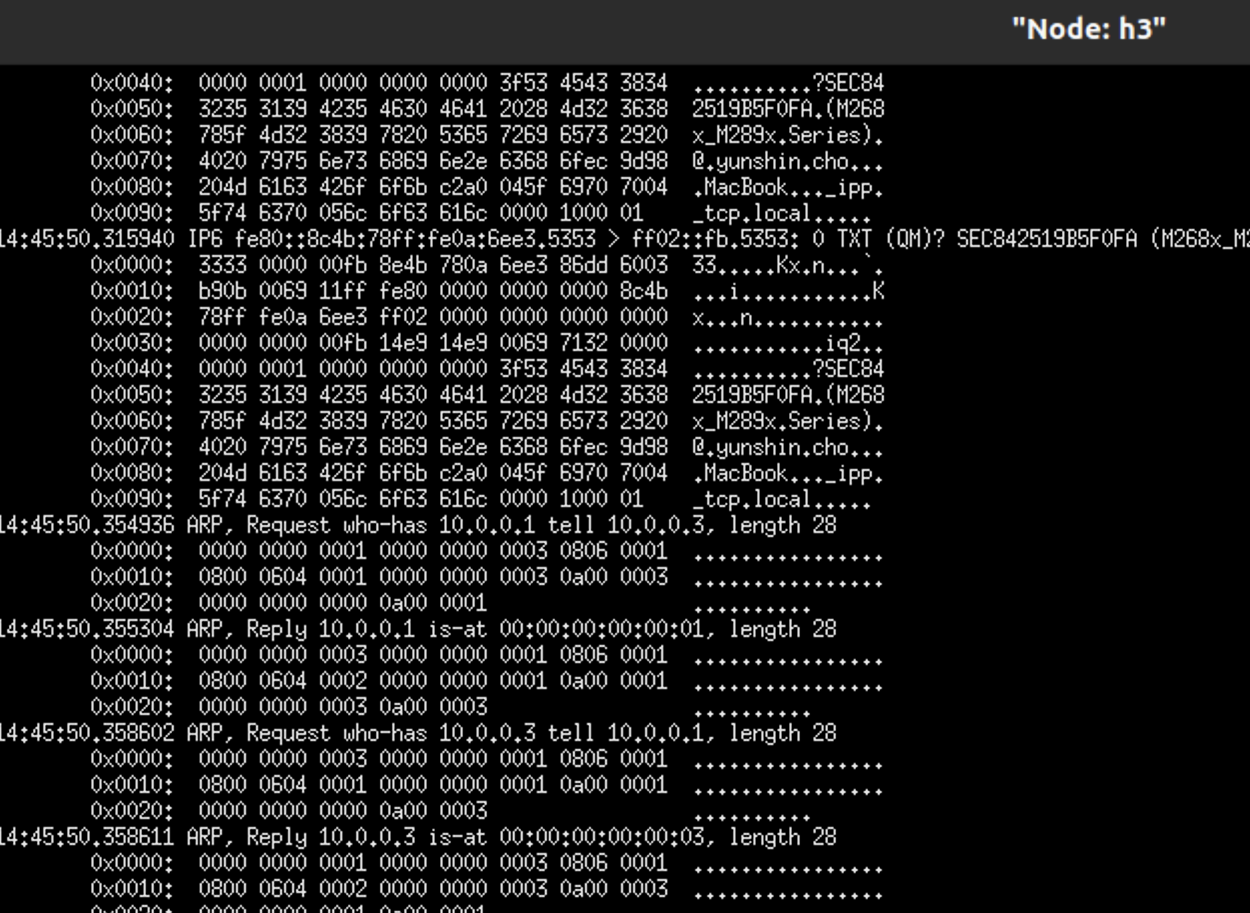
\includegraphics[width=0.33\textwidth]{image/week06/2-3-3.png}
}\caption{}
\end{figure}
\subsubsection{Bandwidth between network hosts}
\begin{figure}[h!]
\centering
\subfloat[]{
    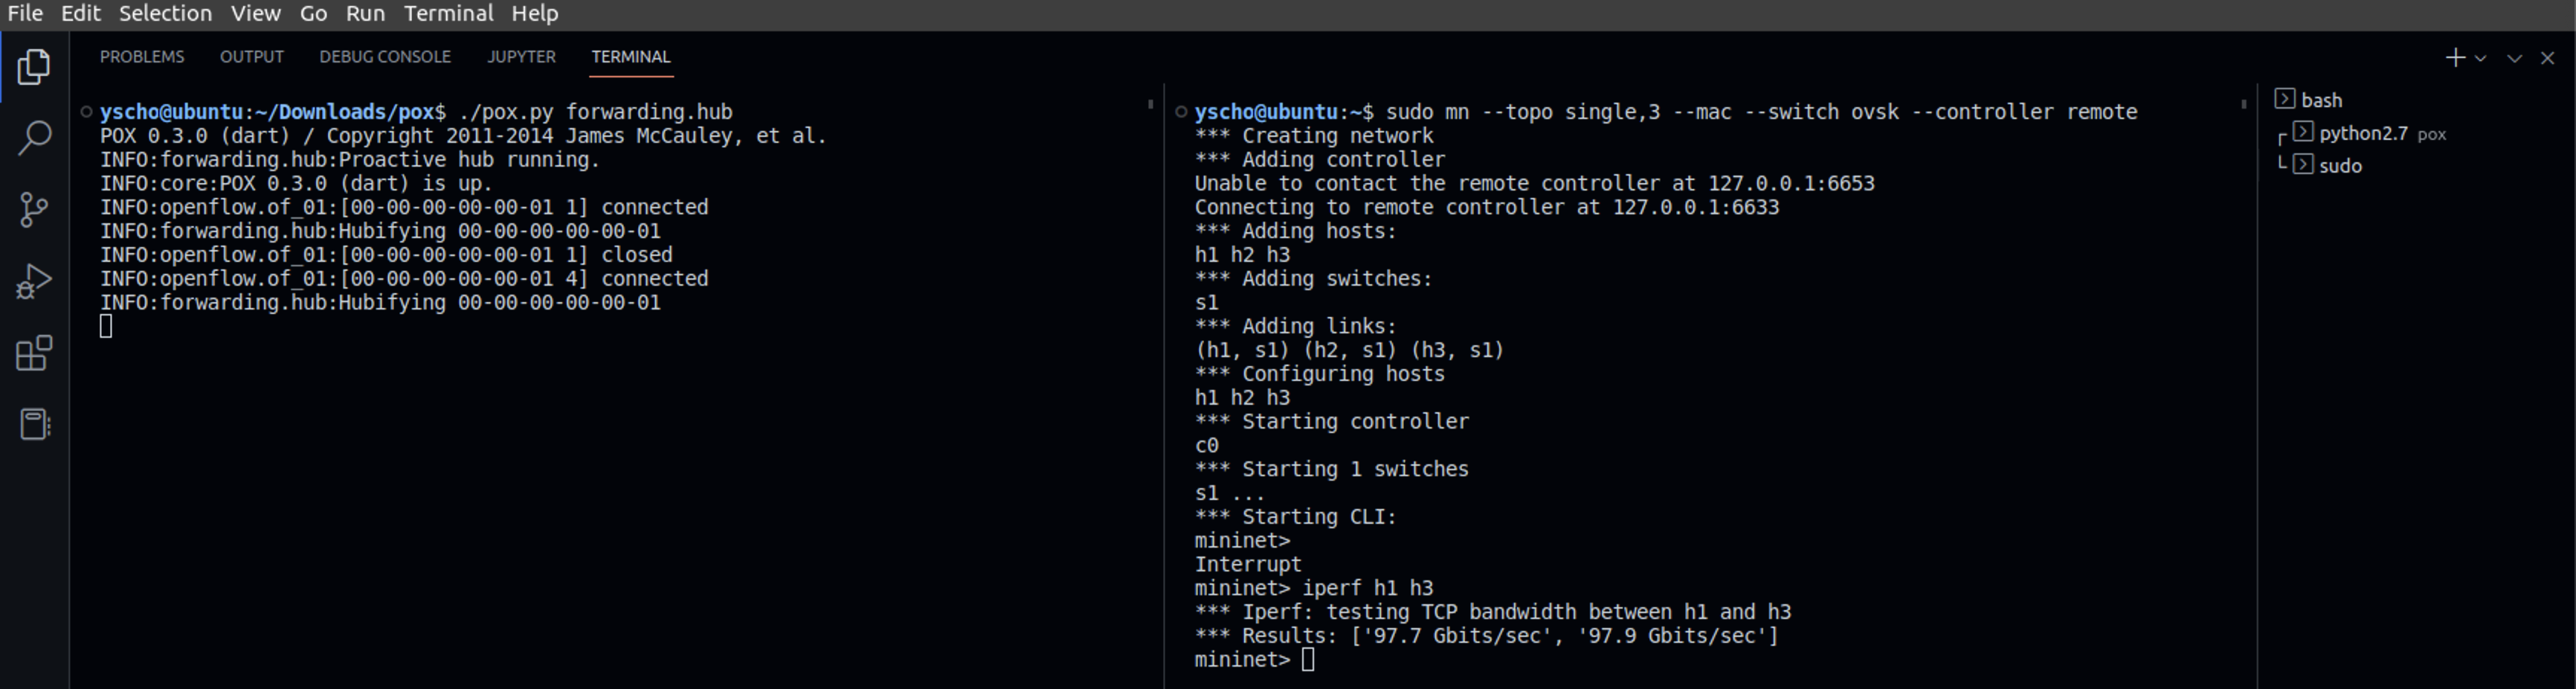
\includegraphics[width=0.99\textwidth]{image/week06/2-4-1.png}
}\hfill
\subfloat[]{
    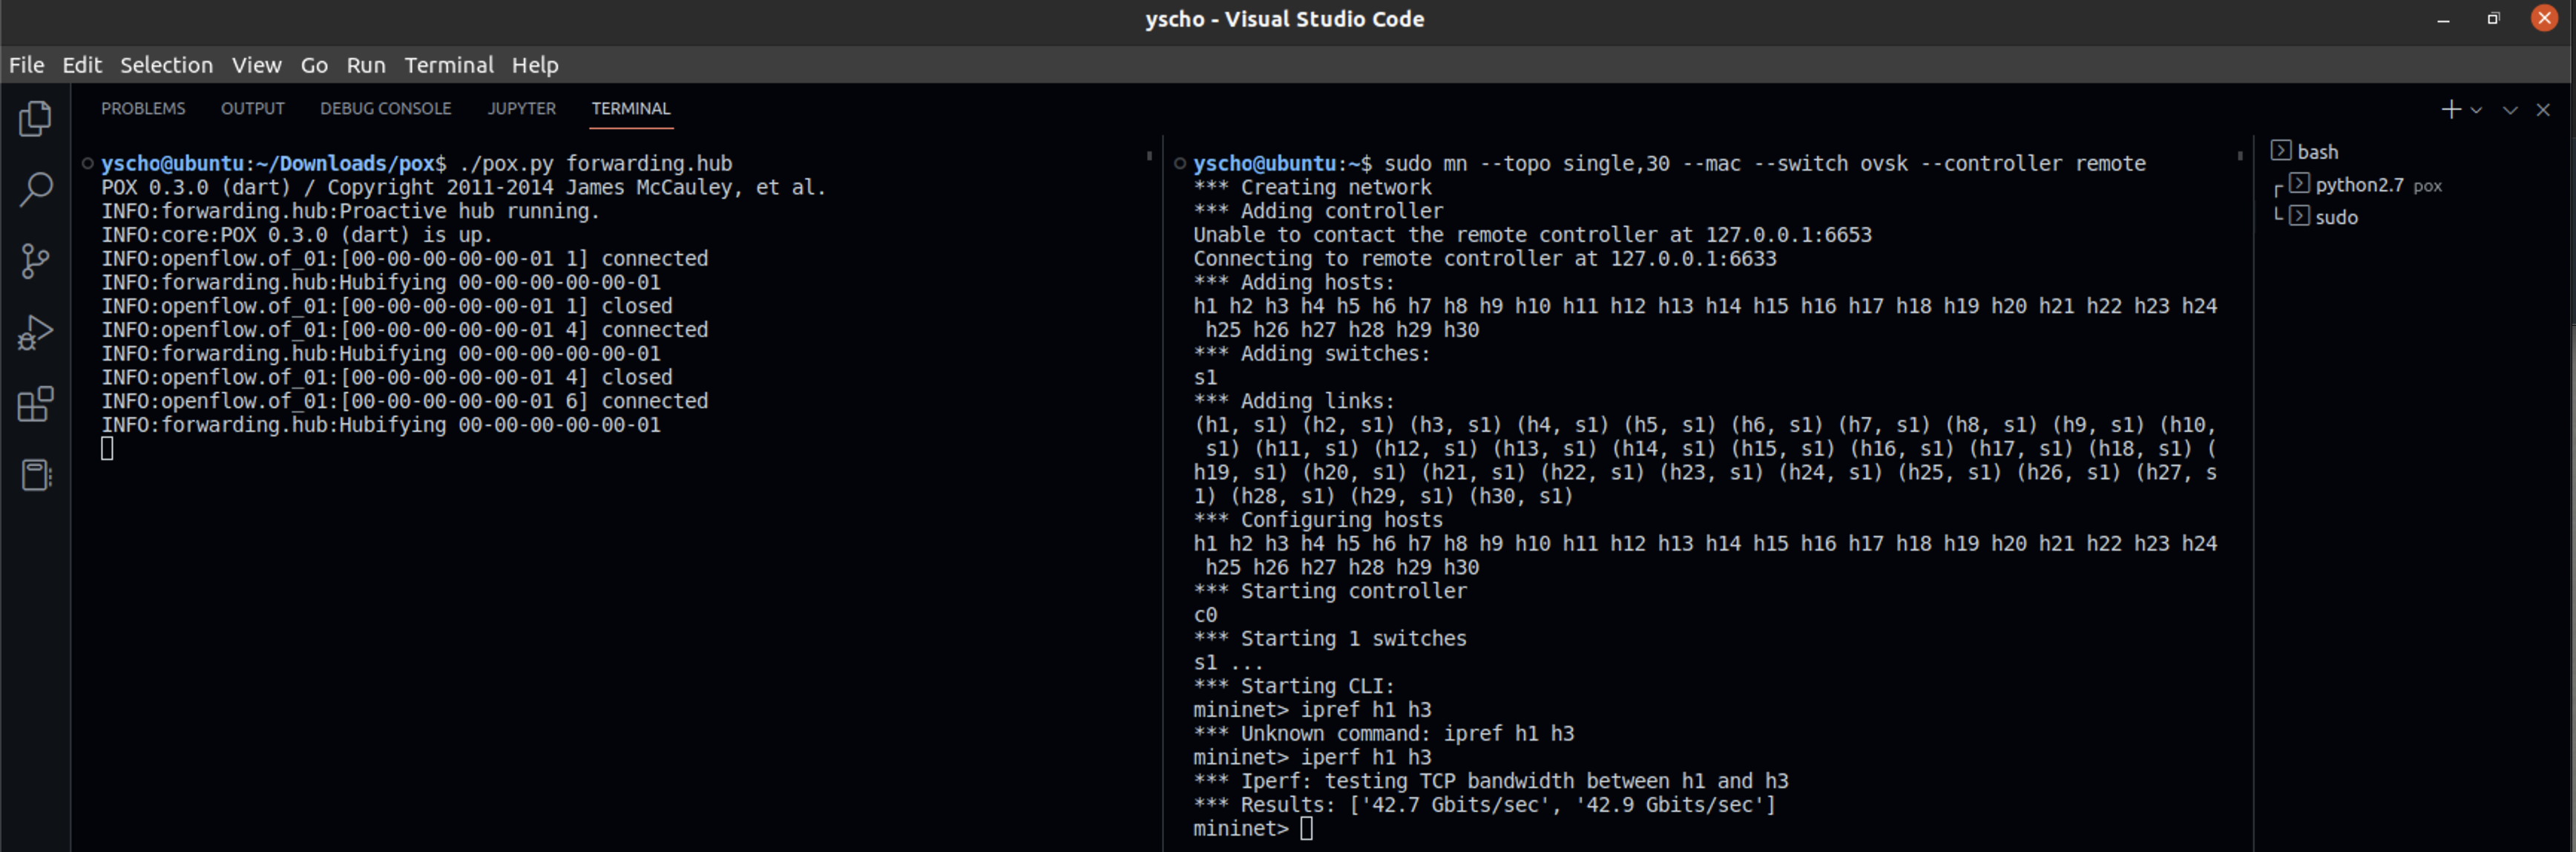
\includegraphics[width=0.99\textwidth]{image/week06/2-4-2.png}
}\hfill
\subfloat[]{
    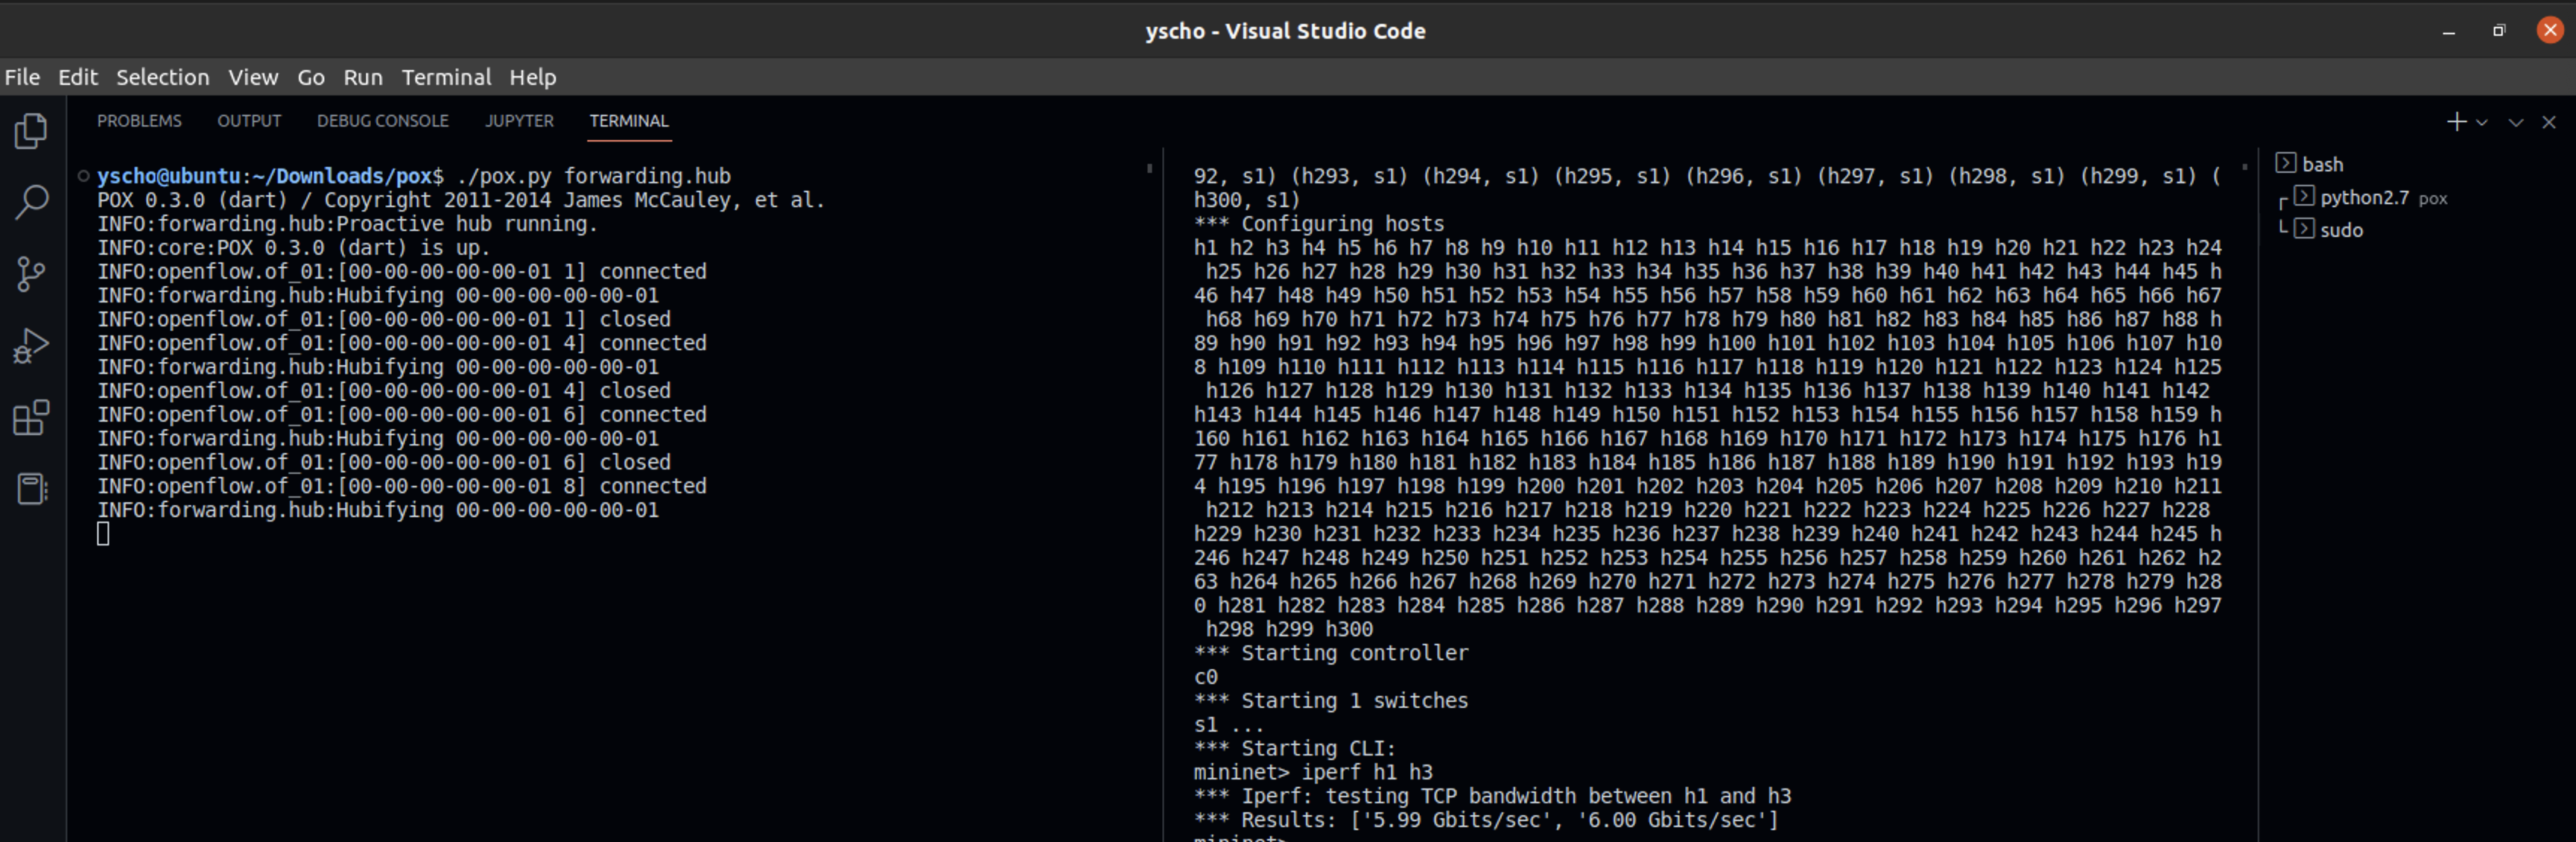
\includegraphics[width=0.99\textwidth]{image/week06/2-4-3.png}
}\caption{}
\end{figure}

\clearpage